%%%%%%%%%%%%%%%%%%%%%%%%%%%%%%%%%%%%%%%%%%%%%%%%%%%%%%%%%%%%%%%%%%%%%%%%%%%%%%%%%%%%%%%%%%%%%%%%%%%
%
% Notes on Citations
%
% MooreAfter2017.bib is an export of the MooreAfter2017 saved search in my Zotero database.
%
% Make sure that the citekey is pinned to each item ( Right click; Better Bibtex | Pin Bibtex key)
%
% After uploading, click on Tools | Bibliography, then open the log file to see any warnings
% or errors which need to be fixed. 
%
% Fix any problems in Zotero, then export a fresh version of MooreAfter2017.bib
%
% Keywords in the MooreAfter2017.bib are used as filters. Note that keywords
% cannot contain space characters.
% 
% Example:
% \begin{refsection}
%	\nocite{*}
%	\printbibliography[heading=none, keyword={Moore-presentations-after-2017}]
% \end{refsection} 
%
%%%%%%%%%%%%%%%%%%%%%%%%%%%%%%%%%%%%%%%%%%%%%%%%%%%%%%%%%%%%%%%%%%%%%%%%%%%%%%%%%%%%%%%%%%%%%%%%%%%
%
% Checking links in PDF
%
% pdfx -c CFES2019.pdf
%
%%%%%%%%%%%%%%%%%%%%%%%%%%%%%%%%%%%%%%%%%%%%%%%%%%%%%%%%%%%%%%%%%%%%%%%%%%%%%%%%%%%%%%%%%%%%%%%%%%%
%
% Subsection format
%
% \begin{refsection}
% \subsubsection{Description}
% \subsubsection{Activities}
% \subsubsection{Plans}
% \subsubsection{References}
% \printbibliography[heading=none]
% \end{refsection}
%
%%%%%%%%%%%%%%%%%%%%%%%%%%%%%%%%%%%%%%%%%%%%%%%%%%%%%%%%%%%%%%%%%%%%%%%%%%%%%%%%%%%%%%%%%%%%%%%%%%%

\documentclass[12pt,english,letterpaper]{scrartcl}
\usepackage[T1]{fontenc}
\usepackage{color}
\usepackage{array}
\usepackage{url}
\usepackage{pdfpages}
\usepackage{longtable}
\usepackage{booktabs}
\usepackage[utf8]{inputenc}
\usepackage[english]{babel}
\usepackage{csquotes}
\usepackage{xcolor}
\usepackage{pgfgantt}

% Use style=draft to print citation keys
% soting=none orders references in the order in which they occur in the document
% maxbibnames=99 prevents use of et al.
\usepackage[sorting=none, style=draft, maxbibnames=99]{biblatex}

% This code adds a category "cited" to cited bibliographic items
\DeclareBibliographyCategory{cited}
\AtEveryCitekey{\addtocategory{cited}{\thefield{entrykey}}}

% IMPORTANT NOTE: Zotero does not provide automatic sync for saved searches. This must be done manually.

\addbibresource{MooreAfter2017.bib}    % From the My Library in my Zotero
\addbibresource{MooreCRBAfter2019.bib} % From the CRB Library in my Zotero
\addbibresource{inat.bib}              % From ?
\addbibresource{misc.bib}              % manually editted
\addbibresource{InPreparation.bib}     % From my Zotero; saved search for "In preparation" in Extras

% Add all build a bibliography containing all references, cited plus uncited
\nocite{*}

\usepackage[breaklinks=true, colorlinks=True, allcolors=blue]{hyperref}

\usepackage{indentfirst} 
\usepackage{comment}

% A couple of very simple macros to add 'Activities' and 'Plans' headings.
\newcommand{\activities}{\medskip\textbf{Activities}}
\newcommand{\plans}{\medskip\textbf{Plans}}

\makeatletter

\makeatother

\errorcontextlines=3 % For checking biblatex

\begin{document}

\title{CFES Report 2020-2022}

\author{Aubrey Moore, Ph.D.\\
Professor / Extension Entomologist}

\maketitle

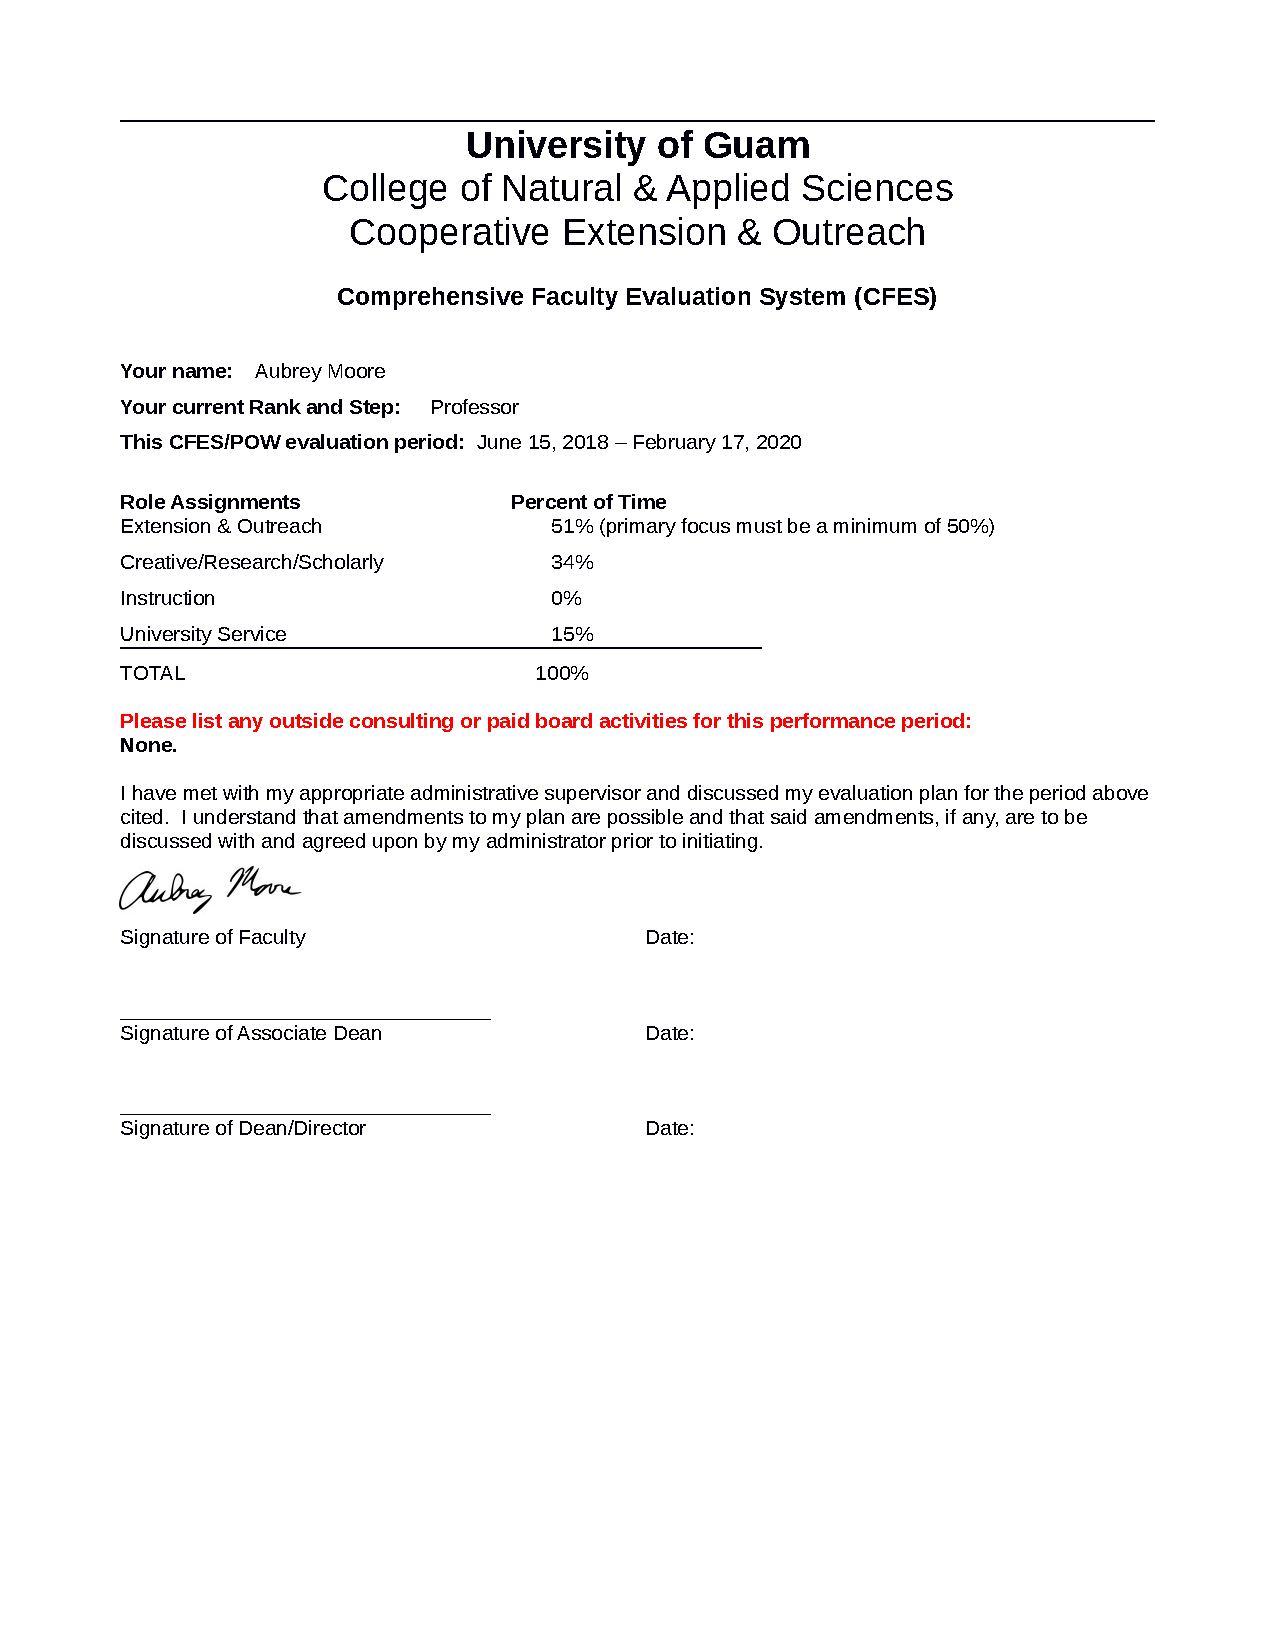
\includepdf[pages=1]{Reflective-form}

\setcounter{tocdepth}{2}
\tableofcontents{}

\clearpage

\section{Preface}

\begin{ganttchart}{1}{12}
	\gantttitle{2011}{12} \\
	\gantttitlelist{1,...,12}{1} \\
	\ganttgroup{Group 1}{1}{7} \\
	\ganttbar{Task 1}{1}{2} \\
	\ganttlinkedbar{Task 2}{3}{7} \ganttnewline
	\ganttmilestone{Milestone}{7} \ganttnewline
	\ganttbar{Final Task}{8}{12}
	\ganttlink{elem2}{elem3}
	\ganttlink{elem3}{elem4}
\end{ganttchart}
	
I was hired by the University of Guam on October 1, 2003 under a limited-term,
split appointment (50\% extension and 50\% research). On June 26,
2008, I started a tenure-track appointment as extension entomologist
(100\% extension) with the academic rank of assistant professor. At
the end of the 2012 fall term I applied for tenure and promotion to associate professor and
received both in 2013. At the end of 2018 fall term I applied for promotion to
full professor and was promoted on July 11, 2019. 

I work within the Agriculture and Natural Resources Unit of the University
of Guam Cooperative Extension Service. I am a faculty member of the
Environmental Science Graduate Program and a member of the Western
Pacific Tropical Research Center. 

This report documents my activities during the period spanning June 15, 2020 to the present date.

My current faculty role allocation is as follows:
\begin{itemize}
	\item 51\% Extension and Community Activities 
	\item 34\% Creative/Scholarly Activity or Research 
	\item 15\% University and Community Service
\end{itemize}

\textbf{Note to Reader:}

This most recent version of this report is available as a PDF format which can be downloaded from \\
\url{https://github.com/aubreymoore/CFES2020-22/raw/main/CFES2020-22.pdf}. 

If you are reading the PDF version of this report on a device connected
to the internet, you will be able to follow hypertext links to documents
I have referenced.

\pagebreak

\section{Extension and Community Activities}

\subsection{Insect Diagnostic Services}
\begin{refsection}

\subsubsection{Description}	
As an extension entomologist, a major part of my job is providing
insect identification and pest control recommendations to a diverse
clientele including commercial growers, gardeners, householders, GovGuam
agencies, federal agencies, and UOG colleagues. Most client contacts
are initiated by a phone call or a visit by the client to the ANR
office. In many cases identification and pest control recommendations
require a site visit by me and/or extension associates to collect
samples and define the problem.

\subsubsection{Activities}

The number of extension calls requiring my assistance averaged approximately
one per day during the reporting period. Many of these are documented
as postings to iNaturalist \cite{moore_inat_since_2020-06-15}.

\subsubsection{Plans}

I plan to continue providing insect diagnostic services.

\subsubsection{References}

\printbibliography[heading=none]
\end{refsection}

\subsection{Detection and Documentation of Invasive Species}
\begin{refsection}

\subsubsection{Description}

Invasive insects are arriving on Guam at a very high rate (estimates
range as high as one new species per day). Very few of these are detected
and even fewer are identified because Guam suffers from \href{https://en.wikipedia.org/wiki/Taxonomic_impediment}{the taxonomic impediment}.
Even when reliable species determinations are made, new island records
are only rarely documented in the scientific press. Thus, impacts
of invasive insects on Guam and elsewhere in Micronesia are grossly
underestimated. One of my professional goals is to work towards solving
this problem by increasing the detection rate, getting specimens identified
by qualified taxonomists, and publishing new island records in the
scientific literature.

\subsubsection{Activities}

iNaturalist was used to document new records for insects detected in Guam and other Micronesian Islands \cite{inatSearch20220327}. 
Four new island records for insects in Micronesia were documented in iNaturalist posts during the reporting period \cite{inat108690775, inat103065598, inat57656025, inat48501627}.

\subsubsection{Plans}

I will continue to document new island records of insects detected in Micronesia.

The International Union for Conservation of Nature (IUCN-ISSG) is
building a Global Register of Introduced and Invasive Species. I have
volunteered to coordinate building a check list for species on Guam.

The Guam Invasive Species Council is required to maintain a list on
invasive species on Guam. I have volunteered to be ``registrar''
for this list.

\subsubsection{References}
\printbibliography[heading=none]
\end{refsection}

\subsection{University of Guam Insect Collection}
\begin{refsection}
	
\subsubsection{Description}

The UOG insect collection is a valuable reference collection for extension
entomology, teaching and research. I am a member of the board of directors
for the collection and I work with Dr. Ross Miller to curate and catalog
this collection.

In 2018 I ported the digital catalog for the UOG Insect Collection from a
CSIRO BioLink database to a more modern web-based Symbiota database
which is publicly available online \cite{moore_scan_2018}. I also established an internship to train entomology students how to curate an institutional insect collection and how to add specimen images to the digital catalog\cite{moore_internship_2018}. However, this work came to a halt because of space limitations. 

Facilities provided for the UOG insect collection are very poor. It is literally \textit{moth balled} in a small storage room which is too small for essential equipment such as microscopes and cameras. Curation and digitization necessitates removing specimens from the collection and transporting them outdoors to a lab where there is working space and equipment.

\subsubsection{Activities}

No significant progress on curation and digitization of the collection has taken place recently because of space limitations.

\subsubsection{Plans}

In 2019 I submitted a proposal for support of the UOG Insect collection as part of the Biorepository Component of the EPSCOR grant \cite{moore_university_2019}. EPSCOR has recently offered up to \$10k in support of the collection. I intend to use this money to temporarily solve the space limitation issue by installing a door to allow access to bench space in the adjoining ANR lab. We already have a quote for this work.

When the space problem has been solved, I intend to re-established the UOG insect collection internship to train entomology students how to curate an institutional insect collection.

\subsubsection{References}
\printbibliography[heading=none]
\end{refsection}

\subsection{Guam Coconut Rhinoceros Beetle Project}

This is my largest and most important project. Please see CRB activities in the Creative/Research/Scholarly section \ref{sec:coconut-rhinoceros-beetle-(crb)-biocontrol}.

\subsection{National Plant Diagnostic Network (NPDN)}
\begin{refsection}

\subsubsection{Description}	

I serve as the UOG Coordinator for the National Plant Diagnostic Network. 

\subsubsection{Activities}

Participated in monthly conference calls.

Prepared an annual work plan and budget \cite{moore_western_2021}.

\subsubsection{Plans}

I will continue to act as UOG coordinator for WPDN.

\subsubsection{References}
\printbibliography[heading=none]
\end{refsection}	

\subsection{Guam Invasive Species Advisory Committee (GISAC) and Guam Invasive Species Council (GISC)}
\begin{refsection}
	
I am a founding member and regular participant in GISAC. President Underwood delegated me to represent UOG as a voting member of GISC and President Krise has reconfirmed my delegation.

\subsubsection{Activities}

I participated in GISAC and GISC meetings.

\subsubsection{Plans}

I plan to continue as an active member of GISAC and GISC.

I plan to participate in a review of the Guam Invasive Species Management Plan.

\subsubsection{References}
\printbibliography[heading=none]
\end{refsection}

\subsection{Public Outreach: Radio and Newspaper}

\begin{refsection}
	\nocite{*}
	\defbibfilter{press}{keyword=press2018 or keyword=press}
	\printbibliography[filter=press, heading=none]
\end{refsection} 

\subsection{Public Outreach: Internet}

Since the 1990s, I have built and maintained web sites to facilitate sharing information about insects in Micronesia. I created a wiki site to serve as an index to web resources I have developed (Available at  \url{https://guaminsects.net/aubwiki2020}). I will continue to use web sites to facilitate sharing information on Guam's insects.

\subsection{Public Outreach: Presentations}
\begin{refsection}
\cite{moore_biological_2021, moore_how_2021}
\subsubsection{References}
\printbibliography[heading=none]
\end{refsection}

\subsection{Public Outreach: Public GitHub Repositories}

I attempt to provide access to as much of my work as possible using public GitHub repositories. GitHub is a free service for backing up and sharing documents on the web. Repositories which I have updated during the reporting period are listed in Table \ref{repolist}. Somewhere near the top of this list you will find a link to a repo called \textbf{CFES2020-22}. This repo contains the this document and all previous versions of the document.

I also use GitHub pages for serving static websites. A couple of good example sites are one which I created for my \href{https://aubreymoore.github.io/ALBI-345/}{ALBI345 General Entomology} course and one which is a \href{https://aubreymoore.github.io/crop-pest-list/}{List of Insects and Mites Attacking Crops in Micronesia}.

\begin{longtable}{ll}
\caption{List of GitHub repositories updated after 2020-06-15.}
\label{repolist}\\
\toprule
   updated &                                                                                                             repo \\
\midrule
\endfirsthead
\caption[]{List of GitHub repositories updated after 2020-06-15.} \\
\toprule
   updated &                                                                                                             repo \\
\midrule
\endhead
\midrule
\multicolumn{2}{r}{{Continued on next page}} \\
\midrule
\endfoot

\bottomrule
\endlastfoot
2022-08-05 &                   \href{https://github.com/aubreymoore/data-mining-insects-of-guam}{data-mining-insects-of-guam} \\
2022-08-04 &                                                   \href{https://github.com/aubreymoore/CFES2020-22}{CFES2020-22} \\
2022-07-30 &                                                                   \href{https://github.com/aubreymoore/POW}{POW} \\
2022-07-29 &                           \href{https://github.com/aubreymoore/2020-DOI-CRB-Biocontrol}{2020-DOI-CRB-Biocontrol} \\
2022-07-18 &                                           \href{https://github.com/aubreymoore/detection-range}{detection-range} \\
2022-07-01 &                   \href{https://github.com/aubreymoore/Guam-Forestry-Workshop-2022}{Guam-Forestry-Workshop-2022} \\
2022-06-30 &                                   \href{https://github.com/aubreymoore/sticky-trap-imaging}{sticky-trap-imaging} \\
2022-06-28 &                                             \href{https://github.com/aubreymoore/albi345-slides}{albi345-slides} \\
2022-06-23 &         \href{https://github.com/aubreymoore/Guam-Forestry-Workshop-Resources}{Guam-Forestry-Workshop-Resources} \\
2022-06-23 &                                                           \href{https://github.com/aubreymoore/crbdist}{crbdist} \\
2022-06-22 &                                                         \href{https://github.com/aubreymoore/CRB-FIDL}{CRB-FIDL} \\
2022-06-22 &                                                                   \href{https://github.com/aubreymoore/CAS}{CAS} \\
2022-06-16 &                                               \href{https://github.com/aubreymoore/gpepp_nursery}{gpepp_nursery} \\
2022-06-16 &                     \href{https://github.com/aubreymoore/sticky_traps_gpepp_nursery}{sticky_traps_gpepp_nursery} \\
2022-06-15 &                                         \href{https://github.com/aubreymoore/2022-06-09-drone}{2022-06-09-drone} \\
2022-05-30 &                                           \href{https://github.com/aubreymoore/good-vibrations}{good-vibrations} \\
2022-05-27 &                                                       \href{https://github.com/aubreymoore/treevibes}{treevibes} \\
2022-05-27 &                                                                 \href{https://github.com/aubreymoore/WPDN}{WPDN} \\
2022-05-25 &                                               \href{https://github.com/aubreymoore/guam-ias-bolo}{guam-ias-bolo} \\
2022-05-17 &                             \href{https://github.com/aubreymoore/CAS-biocontrol-seminar}{CAS-biocontrol-seminar} \\
2022-05-15 &                                                   \href{https://github.com/aubreymoore/inspireguam}{inspireguam} \\
2022-05-13 &                                                   \href{https://github.com/aubreymoore/inat_labels}{inat_labels} \\
2022-05-09 &                                                           \href{https://github.com/aubreymoore/SUMMA21}{SUMMA21} \\
2022-04-27 &                                                         \href{https://github.com/aubreymoore/WPDN2022}{WPDN2022} \\
2022-04-17 &             \href{https://github.com/aubreymoore/Tinian-sticky-traps-2022-02-26}{Tinian-sticky-traps-2022-02-26} \\
2022-04-07 &                                                     \href{https://github.com/aubreymoore/Tinian-CAS}{Tinian-CAS} \\
2022-03-24 &                                   \href{https://github.com/aubreymoore/Tinian-cycad-images}{Tinian-cycad-images} \\
2022-03-16 &                   \href{https://github.com/aubreymoore/Cave-micrographs-2022-03-16}{Cave-micrographs-2022-03-16} \\
2022-02-27 &                     \href{https://github.com/aubreymoore/sticky-trap-image-analysis}{sticky-trap-image-analysis} \\
2022-02-16 &                                             \href{https://github.com/aubreymoore/Harmonic-Radar}{Harmonic-Radar} \\
2021-12-17 &                                         \href{https://github.com/aubreymoore/McIntire-Stennis}{McIntire-Stennis} \\
2021-12-09 &                                           \href{https://github.com/aubreymoore/CRB-PPA19-Final}{CRB-PPA19-Final} \\
2021-12-07 &                         \href{https://github.com/aubreymoore/crb-diet-experiment-2021}{crb-diet-experiment-2021} \\
2021-12-07 &                   \href{https://github.com/aubreymoore/Guam-CRB-Damage-Map-2021-08}{Guam-CRB-Damage-Map-2021-08} \\
2021-12-06 &                                                         \href{https://github.com/aubreymoore/ALBI-345}{ALBI-345} \\
2021-12-04 &                                       \href{https://github.com/aubreymoore/FY19-PPA-Report-1}{FY19-PPA-Report-1} \\
2021-12-03 &                                                         \href{https://github.com/aubreymoore/bug-soup}{bug-soup} \\
2021-11-28 &   \href{https://github.com/aubreymoore/CRB-Action-Group-Webinar-2021-11-23}{CRB-Action-Group-Webinar-2021-11-23} \\
2021-11-27 &                                                   \href{https://github.com/aubreymoore/aubreymoore}{aubreymoore} \\
2021-11-26 &                                                             \href{https://github.com/aubreymoore/Guam05}{Guam05} \\
2021-11-21 &                                                         \href{https://github.com/aubreymoore/MCC-trap}{MCC-trap} \\
2021-10-24 &                                   \href{https://github.com/aubreymoore/github-repos-bibtex}{github-repos-bibtex} \\
2021-10-21 &                                           \href{https://github.com/aubreymoore/SWDC-2021-07-30}{SWDC-2021-07-30} \\
2021-10-19 &                                     \href{https://github.com/aubreymoore/aubrey_nikola_test}{aubrey_nikola_test} \\
2021-10-13 &                                                         \href{https://github.com/aubreymoore/pyzotero}{pyzotero} \\
2021-10-12 &                                                       \href{https://github.com/aubreymoore/GGI-Linux}{GGI-Linux} \\
2021-09-22 &                                           \href{https://github.com/aubreymoore/lecture-mimicry}{lecture-mimicry} \\
2021-09-20 &           \href{https://github.com/aubreymoore/lecture-insect-chemical-ecology}{lecture-insect-chemical-ecology} \\
2021-09-16 &                                                         \href{https://github.com/aubreymoore/open_pos}{open_pos} \\
2021-09-08 &                                                         \href{https://github.com/aubreymoore/groupImg}{groupImg} \\
2021-09-06 &                                                             \href{https://github.com/aubreymoore/mydemo}{mydemo} \\
2021-08-29 &                                             \href{https://github.com/aubreymoore/InsectWingbeat}{InsectWingbeat} \\
2021-08-21 &                                   \href{https://github.com/aubreymoore/Guam-CRB-damage-map}{Guam-CRB-damage-map} \\
2021-08-16 &                           \href{https://github.com/aubreymoore/InsectWingbeatWaveforms}{InsectWingbeatWaveforms} \\
2021-08-08 &                                                         \href{https://github.com/aubreymoore/wingbeat}{wingbeat} \\
2021-08-06 &                               \href{https://github.com/aubreymoore/USFS-Suggestions-2021}{USFS-Suggestions-2021} \\
2021-07-28 &                                       \href{https://github.com/aubreymoore/CRB-Import-Permit}{CRB-Import-Permit} \\
2021-07-22 &                                                 \href{https://github.com/aubreymoore/Pachodynerus}{Pachodynerus} \\
2021-07-13 &                                             \href{https://github.com/aubreymoore/cas-biocontrol}{cas-biocontrol} \\
2021-06-17 &                                                   \href{https://github.com/aubreymoore/cycad-scale}{cycad-scale} \\
2021-06-16 &                                                                 \href{https://github.com/aubreymoore/wiki}{wiki} \\
2021-06-14 &             \href{https://github.com/aubreymoore/2020-FS-CRB-biocontrol-project}{2020-FS-CRB-biocontrol-project} \\
2021-06-09 &                   \href{https://github.com/aubreymoore/top-10-most-costly-ias-mtcc}{top-10-most-costly-ias-mtcc} \\
2021-05-24 &             \href{https://github.com/aubreymoore/worlds-most-costly-ias-on-guam}{worlds-most-costly-ias-on-guam} \\
2021-05-24 &                   \href{https://github.com/aubreymoore/Guam-CRB-Damage-Map-2021-05}{Guam-CRB-Damage-Map-2021-05} \\
2021-05-18 &                                                         \href{https://github.com/aubreymoore/roadside}{roadside} \\
2021-04-24 &                   \href{https://github.com/aubreymoore/Guam-CRB-Damage-Map-2021-03}{Guam-CRB-Damage-Map-2021-03} \\
2021-04-14 &                           \href{https://github.com/aubreymoore/CRB-Project-Update-2021}{CRB-Project-Update-2021} \\
2021-03-29 &                                   \href{https://github.com/aubreymoore/crb-roadside-slides}{crb-roadside-slides} \\
2021-03-22 &                                       \href{https://github.com/aubreymoore/CRB-PPA19-Report3}{CRB-PPA19-Report3} \\
2021-03-22 &                             \href{https://github.com/aubreymoore/online-learning-course}{online-learning-course} \\
2021-03-18 &   \href{https://github.com/aubreymoore/CRB-Action-Group-Webinar-2021-03-17}{CRB-Action-Group-Webinar-2021-03-17} \\
2021-03-13 & \href{https://github.com/aubreymoore/University-of-Guam-Insect-Collection}{University-of-Guam-Insect-Collection} \\
2021-02-21 &                                                         \href{https://github.com/aubreymoore/CRB-CNMI}{CRB-CNMI} \\
2021-02-02 &                                             \href{https://github.com/aubreymoore/bts-mosquitoes}{bts-mosquitoes} \\
2021-01-27 &                   \href{https://github.com/aubreymoore/Guam-CRB-damage-map-2020-12}{Guam-CRB-damage-map-2020-12} \\
2021-01-13 &                     \href{https://github.com/aubreymoore/crb-roadside-impact-report}{crb-roadside-impact-report} \\
2021-01-12 &                                                   \href{https://github.com/aubreymoore/GGI-odonata}{GGI-odonata} \\
2020-12-19 &                                                         \href{https://github.com/aubreymoore/testhtml}{testhtml} \\
2020-12-10 &     \href{https://github.com/aubreymoore/CRBG-action-group-webinar-20201209}{CRBG-action-group-webinar-20201209} \\
2020-12-01 &                                             \href{https://github.com/aubreymoore/py4web-crb-app}{py4web-crb-app} \\
2020-11-24 &                 \href{https://github.com/aubreymoore/CRB-Damage-Survey-Validation}{CRB-Damage-Survey-Validation} \\
2020-11-23 &                                     \href{https://github.com/aubreymoore/new-crb-damage-map}{new-crb-damage-map} \\
2020-11-13 &                   \href{https://github.com/aubreymoore/Guam-CRB-damage-map-2020-10}{Guam-CRB-damage-map-2020-10} \\
2020-11-02 &                                       \href{https://github.com/aubreymoore/USAPI-Mosquito-ID}{USAPI-Mosquito-ID} \\
2020-10-15 &                                                             \href{https://github.com/aubreymoore/Guam01}{Guam01} \\
2020-09-17 &                                         \href{https://github.com/aubreymoore/roadside-article}{roadside-article} \\
2020-09-12 &                                   \href{https://github.com/aubreymoore/roadside-spatialite}{roadside-spatialite} \\
2020-09-04 &                                               \href{https://github.com/aubreymoore/PDF_to_Reveal}{PDF_to_Reveal} \\
2020-08-23 &                                 \href{https://github.com/aubreymoore/CRB-Damage-Detection}{CRB-Damage-Detection} \\
2020-07-10 &                                         \href{https://github.com/aubreymoore/Leo-Palace-Traps}{Leo-Palace-Traps} \\
2020-07-06 &                                                     \href{https://github.com/aubreymoore/qgiswebmap}{qgiswebmap} \\
2020-07-01 &                             \href{https://github.com/aubreymoore/Guam-Corona-Virus-Data}{Guam-Corona-Virus-Data} \\
2020-06-25 &                                 \href{https://github.com/aubreymoore/CRB-trap-improvement}{CRB-trap-improvement} \\
2020-06-21 &                                                                 \href{https://github.com/aubreymoore/temp}{temp} \\
\end{longtable}


\section{Creative/Scholarly Activities or Research}

\subsection{Coconut Rhinoceros Beetle (CRB) Biocontrol}\label{sec:coconut-rhinoceros-beetle-(crb)-biocontrol}
\begin{refsection}
	
\subsubsection{Description}

A newly discovered biotype of coconut rhinoceros beetle (CRB-G) is
rapidly killing coconuts and other palms on Guam and on other Pacific
islands. Following a failed eradication attempt on Guam, CRB-G proved
hard to control because it is resistant to \emph{Oryctes rhinoceros}
nudivirus (OrNV), which was previously used as the preferred biological
control agent for control of CRB outbreaks on Pacific Islands and
elsewhere. Previous to the discovery of CRB-G, all OrNV releases on
Pacific Islands resulted in immediate and sustained suppression of
CRB damage to low levels and prevented tree mortality.

Guam is currently experiencing an uncontrolled and unmonitored island-wide
CRB-G outbreak which was triggered by abundant CRB-G breeding sites
in the form of dead and dying vegetation left in the wake of Typhoon
Dolphin which occured in May 2015. of a recent typhoon. Most of these
breeding sites are inaccessable to sanitation efforts, being either
in the jungle or on military land (which covers one third of Guam).
A positive feedback cycle has begun whereby large numbers of adult
beetles are killing large numbers of palms which become breeding sites
which generate even higher numbers of adults. Severe damage to Guam\textquoteright s
palms prompted the Governor of Guam to declared a state of emergency
in July 2017.

The main objective of this project is to stop the uncontrolled outbreak
on Guam. Entomologists working on the CRB-G problem on several Pacific
islands agree that the most feasible tactic to halt tree mortality
and suppress damage to tolerable levels is establishment of biological
control using an isolate of OrNV which is highly effective as a biological
control agent for CRB-G. We are working with collaborators to identify
populations of CRB-G throughout the Asia-Pacific region. We will sample
these populations for biological control agent candidates which will
be evaluated in laboratory bioassays performed at UOG. Promising candidates
will be field released using autodissemmination as per a USDA-APHIS
import and release permit.

Concurrent with establishment of CRB-G biocontrol, success of the
project will be monitored in a quarterly, island-wide tree health
survey and incidence of OrNV infection will be monitored in a subsample
of all field collected CRB-G.

If the Guam CRB-G infestation cannot be controlled, it is expected
that most palms on the island will be killed and CRB-G will continue
to spread to other islands and beyond. If CRB-G invades smaller islands
and atolls where coconut is the tree of life, a human tragedy will
ensue. On larger islands, coconut and oil palm industries will be
severely impacted. Attempts to organize a regional project in response
to CRB-G are underway.

\subsubsection{Activities}

\paragraph{Funding} This is my largest and most important project, requiring a lot of time and effort for project management including preparation of grant proposals and reports. Funding is currently provided by four grants: USDA-APHIS FY17 Farm Bill~\ref{USDA-APHIS-2017}, USDA-Farm FY18 Bill~\ref{USDA-APHIS-2018}, USDA-Plant Protection Act~\ref{USDA-APHIS-2019} and a grant from the Department of Interior, Office of Insular Affairs~\ref{DOI}. Links to progress reports for these grants are in the appendices. 

I submitted a proposal for FY20 USDA-Plant Protection Act Funds~\ref{USDA-APHIS-2020} and a preproposal for SERDP FY21 funding \ref{SERDP}. 

\paragraph{Staffing}

I am assisted by Dr. James Grasela, and insect pathologist funded by my Department of the Interior Office of Insular Affairs grant \ref{DOI}. Roland Quitugua collaborates on the project with separate funding.  During the reporting period my technician and graduate student, Ian Iriarte, left the University. I have recently hired an entomology student, Christian Cayanan, as a technician.

\paragraph{Current focus} is on finding an isolate of \textit{Oryctes} rhinoceros nudivirus which can be used as a biological control agent for CRB-G. Laboratory bioassays have identified one OrNV isolate which is potential candidate and further tests are under way.

I have developed an online database to facilitate record keeping and report generation for CRB rearing and bioassays \cite{moore_coconut_2019-1}. 

Dr. Grasela has worked in coordination with Dr. Hui Jiang to build DNA diagnostics capacity. We can now test for OrNV in individual beetles.

\paragraph{International collaboration} will be essential for finding a way to halt massive ecological and economic damage to Pacific islands invaded by CRB-G. A CRB-G Action Group has been formed to facilitate collaboration and cooperation.

In August 2018, Moore, Grasela, Quitugua and Iriarte participated in the Congress on Invertebrate Pathology and Microbial Control and the 51st Annual Meeting of the Society for Invertebrate Pathology \cite{moore_trip_2018-1,moore_attempted_2018,marshall_progress_2018}.

During May 2019, Moore travelled to Taiwan to collect CRB-G adults \cite{moore_taipei_2019}. Based on previous research, it seems likely that these beetles will contain OrNV which can be used as a biocontrol agent.

During November 2019, Moore and Grasela participated in the XIX International Plant Protection Congress \cite{moore_india_2019,moore_status_2019,marshall_challenge_2019}.

\paragraph{Outreach} In an effort to facilitate technical and scientific information among people working on CRB, we have developed and maintain several online resources including a wiki \cite{moore_crb-g_2019}, a Facebook site \cite{moore_facebook_2019}, an online interactive map of CRB invasion history \cite{moore_online_2019} and a CRB bibliography \cite{moore_coconut_2019}.

\subsubsection{Plans}

Plans for this project are contingent on applied research results, availability of funding and availability of resources.

\paragraph{Funding} I have submitted a proposal for FY20 USDA-Plant Protection Act Funds~\ref{USDA-APHIS-2020}. A preproposal for 
SERDP resulted in a request for a full proposal due March 4, 2020.  I intend to apply for two more grant proposals to support this project. One to the Department of the Interior Office of Insular Affairs for further support of the insect pathologist postdoctoral position (due April 1, 2020) \ref{doi2} and one to the US Forest Service for a feasibility test of harmonic radar for locating cryptic CRB breeding sites (no deadline) \ref{harmonic radio}.

\paragraph{CRB-G biocontrol} We will continue performing bioassays until a potential OrNV biocontrol candidate is found. Once we have one, we will begin propagation \textit{in vivo} and field releases via autodissemination. I already have a USDA-APHIS permit for field release of OrNV.

\paragraph{Establishment of CRB laboratory colonies} We plan to establish a colony of CRB-G from
Guam and also a colony of CRB-S from American Samoa. We have 3 computer controlled environmental chambers for this purpose and have obtained an permit from USDA-APHIS which allows us to import CRB from American Samoa \cite{usda-aphis_crb_2019,moore_additional_2019}.

We will use beetles reared in these colonies to perform laboratory bioassays will be performed to quantify the toxic (LD50, LT50, etc.)
and nontoxic effects (fecundity, flight capability, etc.) of OrNV on CRB-G.

Beetles from these colonies will also be used to test two hypotheses:
\begin{itemize}
	\item \textbf{Hypothesis 1:} CRB-G has a higher tolerance than CRB-S to OrNV isolates previously used for effective biocontrol. Although CRB-G virus resistance has been presumed, this has not been confirmed
	by comparative bioassays.
	\item \textbf{Hypothesis 2:} CRB-G is less attracted than CRB-S to the synthetic aggregation pheromone, oryc-
	talure. Although CRB pheromone traps baited with oryctalure are widely used, these traps are not
	very attractive to CRB-G on Guam. When marked beetles were released within grids of pheromone
	traps, only 8\% of these were recaptured (Moore, unpublished). We will compare responses of CRB-G
	and CRB-S to oryctalure using a custom-designed y-tube olfactometer and an electroantennogram.
	Dr. Michael Orr and his graduate student, Leilani Sablan are planning to do this work.
\end{itemize}

Once our lab rearing program is established we will provide CRB-S to collaborators, Dr. Madoka Nakai
and Dr. Ross Miller, who are independently investigating the mechanism of virus resistance in CRB-G.

\paragraph{Harmonic radar} I intend to request a small grant from the US Forest Service to test the feasibility of using harmonic radar for locating cryptic CRB breeding sites. This work will be done in collaboration with Dr. Matt Siderhurst, a chemical ecologist at Eastern Mennonite University and it builds on a previous study in which we investigated radio tracking of CRB.

\subsubsection{References}
\printbibliography[heading=none]

\end{refsection}


\subsection{Guam Biodiversity Inventory}
\begin{refsection}
	
	\subsubsection{Description}
	
	I consider this to be my second most important project.
	
	A biodiversity inventory is essentially a database containing a comprehensive
	check list of all taxa known occur within a defined area.
	
	A terrestrial biodiversity inventory for Guam is needed to document
	rapid changes to Guam\textquoteright s ecosystems, to provide free
	and open access to information on Guam\textquoteright s flora and
	fauna, and to share Guam biodiversity information with the global
	scientific community, policy makers and the public.
	
	The Guam Biodiversity Inventory will facilitate automatic generation
	and updates to lists such as: a list of all invasive species on Guam
	with year first recorded, a list of new species described from specimens
	collected on Guam, a list of observations for Guam\textquoteright s
	endangered species, a list of Guam\textquoteright s native plants
	with associated herbivores and pathogens, and a list of crops grown
	on Guam and pests and pathogens which attack them.
	
	\subsubsection{Activities}
	
	Students in my AL/BI 345 class assisted in a project to liberate data from the scientific literature. In this datamining project occurrence records and ecological associates (hosts etc.) for 370 species of insects recorded
	in Insects of Guam I, Bishop Museum Bulletin 172 were extracted. Data extraction was done by 15 entomology student volunteers using free
	crowdsourcing software called Turkle \cite{moore_github_2019-1}. 
	
	\subsubsection{Plans}
	
	I plan to publish the dataset from the above mentioned datamining project as a Darwin core archive, in the Global Biodiversity Information Facility.
	
	I intend to participate in the 4th Annual Digital Data in Biodiversity Research Conference, Bloomington, Indiana, June 1-3, 2020.
	
	\subsubsection{References}
	\printbibliography[heading=none]
\end{refsection}

\subsection{Guam Forest Insect Survey}
\begin{refsection}
	
	\subsubsection{Description}
	
	The objective of this project is to compile a comprehensive check
	list of insects impacting Guam's forests. While it is notable that
	Guam's two most numerous forest trees, namely fadang, \emph{Cycas
		micronesica}, and coconut palm, \emph{Cocos nucifera}, are under simultaneous
	attack by invasive insects, there are many other forest plants under
	attack from invasive insects. This project is funded by McIntire-Stennis.
	
	\subsubsection{Activities}
	
	This grant was completed in 2018. See final report \cite{moore_aubreymoore/mcintire-stennis_2018}.
		
	\subsubsection{Plans}
	
	None. This grant project has been completed.
	
	\subsubsection{References}
	\printbibliography[heading=none]
\end{refsection}


\subsection{Cycad Aulacaspis Scale (CAS) Biocontrol}
\begin{refsection}

\subsubsection{Description}

A US Forest Service survey published in 2002 reported that the most
abundant tree in Guam's forests (DBH > 5 inches) was Guam's endemic
cycad, \emph{Cycas micronesica}. In 2003, an invasive scale insect,
\emph{Aulacaspis yasumatsui,} was detected on ornamental cycads but
it soon infested wild cycads and started killing them. Within a decade,
90\% of Guam\textquoteright s endemic cycads have been killed by the
scale and other invasive species. \emph{Cycas micronesica} was placed
on the US National Endangered Species List in 2015.

Mature plants are protected by a lady beetle I introduced, but no
natural reproduction is occurring because seeds and seedlings are
still being killed by the scale insect. A likely solution to this
problem is establishment of a small biocontrol agent, such as a miniature
parasitic wasp which will control scale insects infesting seeds and
seedlings.

\subsubsection{Activities}

Worked with Ben DeLoso, Tom Marler's grad student, to perform a CAS
parasitoid survey. Results were presented at the Annual Conference of the American Society for Horticulture Science \cite{deloso_parasitoid_2018}.

\subsubsection{Plans}

I plan to write a grant proposal to bring Dr. Ron Cave, an expert on cycad scale biocontrol, as a consultant to provide a plan for dealing with this problem \ref{cycad scale}.

\subsubsection{References}
\printbibliography[heading=none]
\end{refsection}

\subsection{Eight Spot Butterfly (ESB) Conservation}
\begin{refsection}

\subsubsection{Description}

The Guam Department of Agriculture Division of Aquatic and Wildlife
Resources (GDOA-DAWR) requested assistance with conservation of the
rare Mariana eight-spot butterfly, \emph{Hypolimnas octocula marianensis.
}. I prepared a grant proposal and permit application to do this work \cite{aubrey_moore_application_2016} which has been funded \ref{eightspot}.

The objective of this project is to investigate the feasibility of captive rearing.

\subsubsection{Activities}

I have partnered with Dr. Curt (George) Fiedler, Biology Department, and the Center for Island Sustainability to colaborate on this project.

A large field cage (20x20X10 feet) is being built in the CIS compound in Dean's Circle.

\subsubsection{Plans}

Breeding experiments will commence within the next 2 months.

I intend to publish a review article on \textit{Hypolimnas octocula} \cite{moore_mariana_2013}

\subsubsection{References}
\printbibliography[heading=none]
\end{refsection}

\subsection{Development of a Camera Trap for Insects}
\begin{refsection}
\subsubsection{Description}

The objective of this project is to build a camera trap which uses motion detection to automatically capture short videos of active insects.

The initial target application is a surveillance system for insects visiting flowers.

\subsubsection{Activities}

Initial attempts at hardware and software development are available on an Open Science Framework site \cite{moore_development_2019} and in a GitHub repository \cite{moore_github_2019-2}.

\subsubsection{Plans}

For the first target application of this technology, I am partnering with Dr. Jim McConnel and staff of the Guam Plant Extinction Prevention Project to discover insect pollinators of an endangered endemic plant.

I plan to test the camera trap for monitoring bee hive activity, including detecting arrival of hornets (\textit{Vespa tropica}).

USDA-APHIS herpetologist, Dr. Shane Sears, has asked me to collaborate with him on developing digital image analysis of brown tree snake videos.

\subsubsection{References}
\printbibliography[heading=none]
\end{refsection}

\pagebreak
\section{University and Community Service}

\subsection{Instruction}
\begin{refsection}
	
\subsubsection{Description}

In addition to fulfilling my primary role as an extension entomologist, I am required to teach undergraduate courses.

\subsubsection{Activities}

During Fall term 2019, I taught the lecture and laboratory sections of AL/BI 345 General Entomology.

I prepared a syllabus for this course REF. I also built and maintained a web site \cite{moore_web_2019-1} and populated this with lecture notes and other resources.

My scores in the student evaluations of both sections were higher than the university and college averages \cite{moore_student_2019}.

\subsubsection{Plans}

I plan to teach the lecture and laboratory sections on AL/BI 345 in Fall, 2021.

\subsubsection{References}
\printbibliography[heading=none]
\end{refsection}

\subsection{Faculty Committees}

\subsubsection{Faculty Building Facilities Committee for the ALS}

This committee was formed by the Agriculture and Life Sciences Division
to provide advice to the Dean on facilities problems within the Agriculture
and Life Sciences Building. During the reporting period, I was re-elected
as chair of this committee, joined by Dr. Jim McConnell.

\raggedright\vspace{2mm}\textbf{Activity}
	
Plans for improvements to the ALS124 teaching lab have been only partially
achieved. For the past four years, faculty have asked for a dedicated
computer and modern audiovisual equipment to facilitate science teaching. This equipment would also be used for the many workshops conducted in that room.

We continue to struggle with finding solutions to chronic lack of support for maintenance and infrastructure improvement.

\subsubsection{Search Committee: Extension Animal Scientist}

I chaired this committee, joined by Mari Marutani, LaJoy Spears,
Bob Schlub, and Tom Poole, Guam's Territorial Veterinarian. This committee concluded with submission of our recommendation to the Dean on November 20, 2018.

\subsubsection{Search Committee: Extension Agricultural Economist}

I was a member of this committee and I am joined by Bob Barber (chair),
LaJoy Speers, and John Brown. This committee concluded with submission of our recommendation to the Dean during December 2018.

\subsubsection{Search Committee: Research Associate II (CRB Project)}

I chaired this committee and was joined by Jim Grasela, Roland Quitugua,
and Jesse Bamba.

\subsubsection{Continuing Employment Committee: Austin Shelton}

I chaired this committee, joined by Ross Miller and Hui Gong. This committee concluded with submission of our recommendation to the Dean during October 2018. 

\newpage
\section{Grants which were active during the reporting period (n=8)}

\begin{table}[h!]
	\centering
	\caption{List of grants active during the reporting period (2020-06-15 through 2022-06-15).}
	\label{grantlist}
	\begin{tabular}{lp{3in}>{\raggedleft\arraybackslash}l}
		\toprule
		code &                                                                                                    title &  funding \\
		\midrule
		OIA-CRB & Establishment of Self-sustaining Biological Control of Coconut Rhinoceros Beetle Biotype G in Micronesia & \$239,994 \\
		\midrule
		APHIS-CRB &                                        Biological Control of Coconut Rhinoceros Beetle Biotype G on Guam & \$200,000 \\
		\midrule		
		FS-CRB & Establishment of Self-sustaining Biological Control of Coconut Rhinoceros Beetle Biotype G in Micronesia &  \$98,240 \\
		\midrule
		BIODIVERSITY &                                                                       Guam Forest Biodiversity Inventory &  \$80,000 \\
		\midrule		
		WPDN1 &                                                                         Western Plant Diagnostic Network &  \$63,366 \\
		\midrule
		8SPOT &                                                                 Captive Breeding of Eight-spot Butterfly &  \$23,212 \\
		\midrule
		FS-CRB-HR &                         Improving Coconut Rhinoceros Beetle Breeding Site Detection Using Harmonic Radar &  \$23,000 \\
		\midrule
		WPDN2 &                                                                  Western Plant Diagnostic Network FY2022 &  \$15,000 \\
		\bottomrule
	\end{tabular}
\end{table}

\begin{figure}[h!]
\begin{ganttchart}[time slot format=isodate, expand chart=\textwidth]{2020-01-01}{2023-12-31}
%	\gantttitle{2011}{12} \\
	\gantttitlecalendar{year} \\
	\ganttgroup{reporting period}{2020-06-15}{2022-06-15} \\
	\ganttbar{APHIS}{2020-01-01}{2021-08-07} \\
	\ganttbar{DOI-OIA}{2020-06-15}{2023-09-30} \\
	\ganttbar{McStennis}{2020-05-14}{2022-09-30}\\
	\ganttbar{8spot}{2020-01-01}{2022-09-30}\\
	\ganttbar{WPDN1}{2020-01-01}{2021-07-31}\\
	\ganttbar{WPDN2}{2021-09-01}{2022-08-31}\\
	\ganttbar{FS-HR}{2020-06-17}{2022-12-31}\\
	\ganttbar{FS-CRB}{2020-06-17}{2022-12-31}		
	\ganttvrule{}{2020-06-15}
	\ganttvrule{}{2022-06-15}
\end{ganttchart}
\caption{Performance periods for grants which were active during the reporting perion (2020-06-15 through 2022-06-15).}
\end{figure}





\clearpage
\subsection{APHIS-CRB Biological Control of Coconut Rhinoceros Beetle Biotype-G \$200K}
\label{USDA-APHIS-2019}

\subsubsection{Key data}
\begin{itemize}
	\setlength\itemsep{0em}
	\item \textbf{Code:} APHIS-CRB
	\item \textbf{Long title:} Biological Control of Coconut Rhinoceros Beetle Biotype G on Guam	
	\item \textbf{Start date:} 2019-08-08	
	\item \textbf{End date:} \textcolor{red}{2021-08-07}	
	\item \textbf{Total budget:} \$200,000	
	\item \textbf{Federal ID:} AP19PPQS\&T00C168
	\item \textbf{UOG ID:} USDA Biocontrol 2019
	\item \textbf{UOG Account:} 30-2F-311117
	\item \href{https://github.com/aubreymoore/FY19-PPA-Report-1}{GitHub repository}
\end{itemize}

\subsubsection{Documents}
\begin{itemize}
	\setlength\itemsep{0em}	
	\item \href{https://github.com/aubreymoore/Miscellaneous-Docs-for-CFES2018/raw/master/MooreFB19.pdf}{Proposal}		
	\item \href{https://github.com/aubreymoore/FY2018-Farm-Bill-Suggestion/blob/master/from\%20EFG/Award\%20Document.pdf}{Award letter}			
	\item \href{https://github.com/aubreymoore/FY2018-Farm-Bill-Suggestion/raw/master/extension-request/MooreFB19WorkPlan-ammended.pdf}{Ammended work plan}		
	\item \href{https://github.com/aubreymoore/FY19-PPA-Report-1/raw/master/PPA19-report-1.pdf}{Report 1}	
	\item \href{https://github.com/aubreymoore/FY19-PPA-Report-1/raw/master/PPA19-report2.pdf}{Report 2}		
	\item \href{https://github.com/aubreymoore/CRB-PPA19-Report3/blob/main/PPA19-report3.pdf}{Report 3}		
	\item \href{}{Final Report}
\end{itemize}




\clearpage
\subsection{OIA-CRB Biological Control of Coconut Rhinoceros Beetle Biotype-G in Micronesia \$177K}
\label{DOI}

\subsubsection{Key data}
\begin{itemize}
	\setlength\itemsep{0em}	
	\item \textbf{Code:} OIA-CRB
	\item \textbf{Title:} Establishment of Self-sustaining Biological Control of Coconut Rhinoceros Beetle Biotype G in Micronesia
	\item \textbf{Start date:} 2020-05-14
	\item \textbf{End date:} 2023-09-30
	\item \textbf{Total budget:} \$239,994
	\item \textbf{Federal ID:} D20AP00060
	\item \textbf{UOG ID:} DOI Biocontrol CRB
	\item \textbf{UOG Account:} 30-2F-311150
	\item \href{https://github.com/aubreymoore/2020-DOI-CRB-Biocontrol}{GitHub repository}
\end{itemize}

\subsubsection{Documents}
\begin{itemize}
	\setlength\itemsep{0em}	
	\item \href{https://github.com/aubreymoore/2020-DOI-CRB-Biocontrol/blob/master/doi_proposal.pdf}{Proposal}
	\item \href{https://github.com/aubreymoore/2020-DOI-CRB-Biocontrol/blob/master/D20AP00060-Grant\%20Award\%20Document.pdf}{Award letter}
	\item \href{https://github.com/aubreymoore/2020-DOI-CRB-Biocontrol/raw/master/Reporting\%20requirements\%20\%20D17AP00107.pdf}{Reporting requirements}
	\item \href{https://github.com/aubreymoore/2020-DOI-CRB-Biocontrol/raw/master/doi_report1.pdf}{Report 1}
\end{itemize}

\newpage
\subsection{BIODIVERSITY Guam Forest Biodiversity Inventory \$80K}

\subsubsection{Key data}
\begin{itemize}
	\setlength\itemsep{0em}
	\item \textbf{Code:} BIODIVERSITY
	\item \textbf{Title:} Guam Forest Biodiversity Inventory
	\item \textbf{Funding source:} McIntire-Stennis (administered by CNAS)
	\item \textbf{Reporting system:} \href{https://portal.nifa.usda.gov/portal/front/login}{REEport}
	\item \textbf{Start date:} 2018-10-15
	\item \textbf{End date:} 2022-09-30
	\item \textbf{Total budget:} \$16,000 per year for each of 4 years
	\item \textbf{Federal ID:} GUA0930
	\item \textbf{UOG ID:}
	\item \textbf{UOG Account:}
	\item \href{https://github.com/aubreymoore/McIntire-Stennis}{GitHub repository}
\end{itemize}

\subsubsection{Documents}
\begin{itemize}
	\setlength\itemsep{0em}	
	\item \href{https://github.com/aubreymoore/McIntire-Stennis/raw/master/MS_Project_Proposal_2018/ms_proposal_2018.pdf}{2018-06-21 Proposal}
	\item \href{https://github.com/aubreymoore/McIntire-Stennis/raw/master/project_initiation.pdf}{2018-10-08 Project initiation}
	\item \href{https://github.com/aubreymoore/McIntire-Stennis/raw/master/2019-report.pdf}{2020-01-02 2019 Annual report}
	\item \href{https://github.com/aubreymoore/McIntire-Stennis/raw/master/2020\%20Annual\%20Report/2020\%20McS\%20Annual\%20Report.pdf}{2020-12-28 2020 Annual report}
	\item \href{}{Annual report due 2021-12-31}
	\item \href{}{Final report due 2022-12-31}
\end{itemize}





\newpage
\subsection{8SPOT Eight Spot Butterfly Conservation \$20K}
\label{eightspot}
\subsubsection{Key data}
\begin{itemize}
	\setlength\itemsep{0em}
	\item \textbf{Code:} 8SPOT
	\item \textbf{Title:} Captive Breeding of Eight-spot Butterfly
	\item \textbf{Start date:} 2013-10-01
	\item \textbf{End date:} 2022-09-30
	\item \textbf{Total budget:} \$23,212
	\item \textbf{Funding Agency:} DOI-FWS (via GDOA-DAWR)
	\item \textbf{Federal ID (FAIN):} F13AF01300
	\item \textbf{UOG ID:}
	\item \textbf{UOG Account:} 30-1F-315058-R
	\item \href{https://github.com/aubreymoore/Hypolimnas-octocula-conservation}{GitHub repository}
\end{itemize}

\subsubsection{Documents}
\begin{itemize}
	\setlength\itemsep{0em}	
	\item \href{https://github.com/aubreymoore/Hypollimnas-octocula-conservation/blob/master/8spot-award-notice.pdf}{Award letter (includes scope of work and budget)}
	\item \href{https://github.com/aubreymoore/Hypollimnas-octocula-conservation/blob/master/8spot-award-notice-updated.pdf}{Updated Award Letter}
	\item \href{}{Report 1; performance period; due on}
\end{itemize}





\newpage
\subsection{WPDN1 Western Plant Diagnostic Network 2016 \$63K}
\label{WPDN}

\subsubsection{Key data}
\begin{itemize}
	\setlength\itemsep{0em}	
	\item \textbf{Code:} WPDN1
	\item \textbf{Long title:} Western Plant Diagnostic Network
	\item \textbf{Start date:} 2016-09-01
	\item \textbf{End date:} \textcolor{red}{2021-07-31}
	\item \textbf{Total budget:} \$63,366
	\item \textbf{Federal ID(FAIN):} 20163762025851
	\item \textbf{UOG ID:}
	\item \textbf{UOG Account:} 2F-243432R5
	\item \href{https://github.com/aubreymoore/WPDN}{GitHub repository}
\end{itemize}

\subsubsection{Documents}
\begin{itemize}
	\setlength\itemsep{0em}	
	\item \href{https://github.com/aubreymoore/WPDN/raw/main/WPDN\%20-award-2020.pdf}{Proposal and Award Letter}
	\item \href{}{Report 1; performance period; due on YYYY-MM-DD}
\end{itemize}





\newpage
\subsection{WPDN2 Western Plant Diagnostic Network FY2022 \$15K}
\label{WPDN}

\subsubsection{Key data}
\begin{itemize}
	\setlength\itemsep{0em}	
	\item \textbf{Code:} WPDN2
	\item \textbf{Title:} Western Plant Diagnostic Network FY2022
	\item \textbf{Start date:} 2021-09-01
	\item \textbf{End date:} 2022-08-31
	\item \textbf{Total budget:} \$15,000
	\item \textbf{UOG ID:} WPTRC-UCDAVIS/USDA WPLANTDI
	\item \textbf{UOG Account:} 61-1F-243432
	\item \href{https://github.com/aubreymoore/WPDN}{GitHub repository}
\end{itemize}

\subsubsection{Documents}
\begin{itemize}
	\setlength\itemsep{0em}	
	\item \href{https://github.com/aubreymoore/WPDN/blob/main/WPDN\%202021-2022\%20workplan\%20and\%20budget.pdf}{Work plan and budget}
	\item \href{https://github.com/aubreymoore/WPDN/raw/main/FY2022/WPDN-FY2022-Award-Letter.pdf}{Award letter}
	\item \href{https://github.com/aubreymoore/WPDN/raw/main/FY2022/UOG-account-setup.pdf}{UOG account setup}
\end{itemize}





\newpage
\subsection{FS-CRB-HR Harmonic Radar \$23K}
\label{2020FS-CRB}

\subsubsection{Key data}
\begin{itemize}
	\setlength\itemsep{0em}
	\item \textbf{Code:} FS-CRB-HR
	\item \textbf{Long title:} Improving Coconut Rhinoceros Beetle Breeding Site Detection Using Harmonic Radar
	\item \textbf{Start date:} 2020-06-17
	\item \textbf{End date:} 2022-12-31
	\item \textbf{Total budget:} \$23,000
	\item \textbf{Federal ID:} 20-DG-11052021-227
	\item \textbf{UOG ID:} CNAS-USDA-CRB Harmonic Radar
	\item \textbf{UG Account:} 30-2F-311144-R
	\item \href{https://github.com/aubreymoore/Harmonic-Radar}{GitHub repository}
\end{itemize}

\subsubsection{Documents}
\begin{itemize}
	\setlength\itemsep{0em}		
	\item \href{https://github.com/aubreymoore/Harmonic-Radar/blob/master/USFS-harmonic-radar-proposal.pdf}{Proposal}
	\item \href{https://github.com/aubreymoore/grant-tracker/blob/main/mydocs/20-DG-227-UOG-CRB-Harmonic-Radar-Fully-Signed-Grant.pdf}{Award letter}
	\item \href{https://github.com/aubreymoore/grant-tracker/blob/main/mydocs/20-DG-227\%20UOG\%20Mod\%201\%20Fully\%20Signed.pdf}{Extension until 2022-12-31}
	\item \href{https://github.com/aubreymoore/Harmonic-Radar/raw/master/FS-CRB-HR-report1.pdf}{Report 1 (2021-01-31)}
	\item \href{}{Report 2 (2021-07-31)}
	\item \href{}{Final report (90 days after expiration date)}
\end{itemize}





\newpage
\subsection{Forest Service CRB \$98K}
\label{2020FS-CRB}

\subsubsection{Key data}
\begin{itemize}
	\setlength\itemsep{0em}	
	\item \textbf{Code:} FS-CRB
	\item \textbf{Long title:} Establishment of Self-sustaining Biological Control of Coconut Rhinoceros Beetle Biotype G in Micronesia
	\item \textbf{Start date:} 2020-06-17
	\item \textbf{End date:} 2022-12-31
	\item \textbf{Total budget:} \$98,240
	\item \textbf{Federal ID:} 20-DG-11052021-229
	\item \textbf{UOG ID:} CNAS-USDA Control of CRB
	\item \textbf{UG Account:} 30-2F-311143-R
	\item \href{https://github.com/aubreymoore/2020-FS-CRB-biocontrol-project}{GitHub repository}
\end{itemize}

\subsubsection{Documents}
\begin{itemize}
	\setlength\itemsep{0em}	
	\item \href{https://github.com/aubreymoore/2020-FS-CRB-biocontrol-project/blob/master/combined-proposal.pdf}{Proposal}
	\item \href{https://github.com/aubreymoore/grant-tracker/blob/main/mydocs/20-DG-229\%20UOG\%20LFA\%20CRB\%20Fully\%20Signed\%20Grant.pdf}{Award letter}
	\item \href{https://github.com/aubreymoore/grant-tracker/blob/main/mydocs/20-DG-229\%20UOG\%20Mod\%201\%20Fully\%20Signed.pdf}{Extension until 2022-12-31}
	\item \href{https://github.com/aubreymoore/2020-FS-CRB-biocontrol-project/raw/master/FS-CRB-biocontrol-report1.pdf}{Report 1 (2021-01-31)}
	\item \href{}{Report 2 (2021-07-31)}
	\item \href{}{Final report}
	\item \href{https://github.com/aubreymoore/2020-FS-CRB-biocontrol-project/blob/master/20-DG-229-UOG-Mod-2-Fully-Signed.pdf}{2021-06-15 Amended agreement}
\end{itemize}





\newpage
\section{Submitted Grant Proposals (n=2)}

\subsection{USDA-APHIS-2020 Biological Control of Coconut Rhinoceros Beetle Biotype-G 1Y \$331K}
\label{USDA-APHIS-2020}
\begin{refsection}
Proposal \cite{moore_fy20_2019};
Budget \cite{moore_fy20_2019-1} 
\printbibliography[heading=none]
\end{refsection}

\subsection{SERDP Biological Control of Coconut Rhinoceros Beetle in the American Pacific 4Y \$3.6M}
\label{SERDP}
\begin{refsection}
Answers to \textit{pitch questions} \cite{moore_aubreymoore/answers--pitch-questions_2019}; 
Preproposal \cite{moore_serdp_2020}	
\printbibliography[heading=none]
\end{refsection}

\newpage

\section{Grant Proposals in Preparation (n=3)}

\subsection{USFS Harmonic Radar}
\label{harmonic radio}
\begin{refsection}

We plan to submit this proposal to the US Forest Service and to publish it in Research Ideas and Outcomes Journal \cite{moore_improving_nodate}. Here is the lead paragraph:

The coconut rhinoceros beetle, Oryctes rhinoceros L., is a serious pest of coconut and other palms throughoutSoutheast Asia and on several Pacific Islands including Hawaii and Guam.  One of the major hurdles for eradication and control of CRB is the location of cryptic breeding sites.  While searching for cryptic breeding sites can be conducted by both humans and dogs, each of these search methods have drawbacks.  Supported by a previous US Forest Service grant, we successful developed a third detection method for cryptic CRB breeding sites using radio-tagged CRB (a so-called "Judas beetle" method).  However, there are both financial (radio tags are expensive) and logistic (radio tags have both limited field- and shelf-life) issues with radio-tracking.  A cheaper and longer lasting alternative to radio-tracking is harmonic radar, which uses cheaper tags that have a near infinite operational lifetime but have a shorter range and more limited available tracking frequencies.  We have recently been successful in using harmonic radar to track the spotted lanternfly, Lycorma delicatula, and are eager to employ this technology to locate cryptic CRB breeding sites.  We propose to develop a harmonic radar tag based CRB tracking system to provide a more cost-effective method for finding cryptic breeding sites, therefore providing a needed tool for CRB eradication and control.

\printbibliography[heading=none]
\end{refsection}

\subsection{USFS Biological Control of Cycad Scale}
\label{cycad scale}

I intend to write a small grant proposal to request funding from the US Forest Service to bring Dr. Ron Cage, an expert on biological control of Asian cycad scale, to Guam as a consultant to provide recommendations.

\subsection{DOI-OIA Biological Control of Coconut Rhinoceros Beetle in the American Pacific}
\label{doi2}

I intend to write a grant to the Department of Interior Office of Insular Affairs requesting continued support for Biological Control of Coconut Rhinoceros Beetle in the American Pacific.

\pagebreak

\section{Journal Articles in Preparation (n=7)}
\begin{refsection}
	
\cite{moore_first_nodate-1,moore_mariana_2013,moore_three_nodate-1,moore_change_nodate,moore_aubrey_crb_nodate,marshall_recent_nodate,moore_coconut_nodate-1}

\printbibliography[heading=none]
\end{refsection}

\section{Uncited References}
This section should be commented out when the report is completed.
\printbibliography[heading=none, notcategory=cited]


\end{document}
